\documentclass{article}

\usepackage{graphicx}
\usepackage{subfigure}
\usepackage{algorithm}
\usepackage{algorithmic}

\usepackage{hyperref}
\newcommand{\theHalgorithm}{\arabic{algorithm}}

% Employ this version of the ``usepackage'' statement after the paper has
% been accepted, when creating the final version.  This will set the
% note in the first column to ``Appearing in''
% \usepackage[accepted]{icml2011}

\usepackage[accepted]{icml2011}

\usepackage{xcolor}
\usepackage[american]{babel}
\usepackage{auto-pst-pdf}
\usepackage{microtype}
\usepackage{psfrag}
\usepackage{amsmath}
\usepackage{amssymb}
\usepackage{pst-all}
%\usepackage[T1]{fontenc}
\usepackage{nicefrac}
\usepackage{booktabs}
\usepackage{pst-all}

\usepackage{natbib}

\newcommand{\psff}[1]{\input{#1.tex}\includegraphics{#1.eps}}
\newcommand{\R}{\ensuremath{\mathbb{R}}}
\newcommand{\deq}{\ensuremath{\triangleq}}
\newcommand{\given}{\ensuremath{\mid}}
\newcommand{\cm}[1]{\ensuremath{\mathcal{#1}}}
\newcommand{\bm}[1]{\ensuremath{\mathbf{#1}}}
\newcommand{\data}{\ensuremath{\cm{D}}}
\newcommand{\inv}{\ensuremath{^{-1}}}
\newcommand{\acro}[1]{\textsc{#1}}

% Mike's definitions
\newcommand{\dd}[2]{\delta(#1-#2))}
\newcommand{\vect}[1]{\bm{#1}}
\newcommand{\vy}{\vect{y}}
\newcommand{\vx}{\vect{x}}
\newcommand{\vf}{\vect{f}}
\newcommand{\vs}{\vect{\sigma}}
\newcommand{\amean}[2]{\tilde{{m}}(#1 \given #2 )}
\newcommand{\acov}[2]{\tilde{{C}}(#1 \given #2 )}
\newcommand{\p}[2]{p(#1\given#2)}
\newcommand{\fPr}{p}
\newcommand{\Prob}[2]{\fPr(#1 \given #2 )}
\newcommand{\ps}[2]{p(#1\vert#2)}
\newcommand{\mean}[2]{{m}(#1\given#2)}
\newcommand{\cov}[2]{{C}(#1\given#2)}
\newcommand{\N}[3]{\cm{N}( #1;#2,#3 )}
\newcommand{\st}{_{\star}}
\newcommand{\tr}{\ensuremath{\mathsf{T}}}
\DeclareMathOperator{\fault}{fault}
\DeclareMathOperator{\diag}{diag}
\DeclareMathOperator{\chol}{chol}

\icmltitlerunning{Environmental Monitoring and Water Sustainability}

\nonstopmode

\begin{document}

\twocolumn[ 

  \icmltitle{A Machine Learning Approach to Pattern Detection and Prediction for
Environmental Monitoring and Water Sustainability}

  \icmlkeywords{Gaussian processes, time-series prediction, fault
    detection, pattern detection, hyperparameter marginalization, water sustainability, environmental monitoring}
    
\icmlauthor{Michael Osborne$^\ast$}{mosb@robots.ox.ac.uk}
\icmlauthor{Roman Garnett$^\dagger$}{rgarnett@andrew.cmu.edu}
\icmlauthor{Kevin Swersky$^\ddagger$}{kevin@aquaticinformatics.com}
\icmlauthor{Nando de Freitas$^\text{\S}$}{nando@cs.ubc.ca}
\icmladdress{$^\ast$Department of Engineering Science, University of Oxford \vspace{-10pt}}
\icmladdress{$^\dagger$Department of Computer Science, Carnegie Mellon University \vspace{-10pt}}
\icmladdress{$^\ddagger$Aquatic Informatics \vspace{-10pt}}
\icmladdress{$^\text{\S}$Department of Computer Science, University of British Columbia}

\vskip 0.3in
]

\begin{abstract}
We describe one of the successful products of a research partnership among several academic institutions (CMU, Oxford and UBC) and a water monitoring company (Aquatic Informatics). Water monitoring sensors are very diverse and remotely distributed. They produce vast quantities of data. The data itself is nonlinear and nonstationary. In addition, unanticipated environmental conditions and limitations in the sensing and communications hardware cause the data to be corrupted by previously uncharacterized nonlinearities, missing observations, spikes and multiple discontinuities. To improve the quality of the data and the monitoring process, this paper introduces an approach that uses Gaussian processes and a general ``fault bucket'' to capture \textit{a priori} uncharacterized faults, along with an approximate method for marginalizing the potential faultiness of all observations. This gives rise to an efficient, flexible algorithm for the detection and automatic correction of faults. The probabilistic nature of the method is ideal for reporting uncertainty estimates to human operators.
The approach can also be applied to detect patterns, other than faults, which are of great environmental significance. We present a fish sustainability example, where specific patterns in water level need to be detected so that fish don't get trapped and die in shallow pools.
\end{abstract}

\section{Introduction}

Water sustainability is one of the greatest challenges that humankind
faces. It is also a problem to which the machine-learning community
can make positive, significant contributions. Water sustainability
begins with proper water monitoring, which requires the analysis and
interpretation of vast amounts of environmental data
\citep{wagner2006guidelines}. We refer readers to the website of Aquatic Informatics\footnote{www.aquaticinformatics.com} for a broad picture of water monitoring. 

In this paper, we attack the problem of
pattern detection, correction, and prediction in water monitoring
signals.  Here measurements are often corrupted in non-trivial ways by
various intermittent faulty sensing and communication mechanisms,
giving rise to outliers, telemetry spikes, missing data, drift, and
multiple unanticipated exogenous disturbances (see
Figure~\ref{fig:monitoring}).  Further, signals are not well-modelled
by simple parametric approaches, such as linear or Markovian
models. Despite the enormous importance of such monitoring,
appropriate machine-learning techniques are yet to be deployed for
this purpose. In particular, there is a clear need for flexible
algorithms, able to cope with signals and faults of many different
types without placing a significant model-building burden upon
users. Such algorithms must also be able to run reliably in real-time
on incoming data.
% To accomplish this, we need to design
% techniques for detecting patterns and making predictions with
% challenging datasets, fraught with 
% %missing data, discontinuities and
% \textit{a priori} unknown types of nonlinearity and non-stationarity.
These techniques will enable us to provide operators with high-level
summaries for better decision support and, in the future, to increase
the level of automation and efficiency in water-management systems.

\begin{figure*}[t!]
\begin{center}
 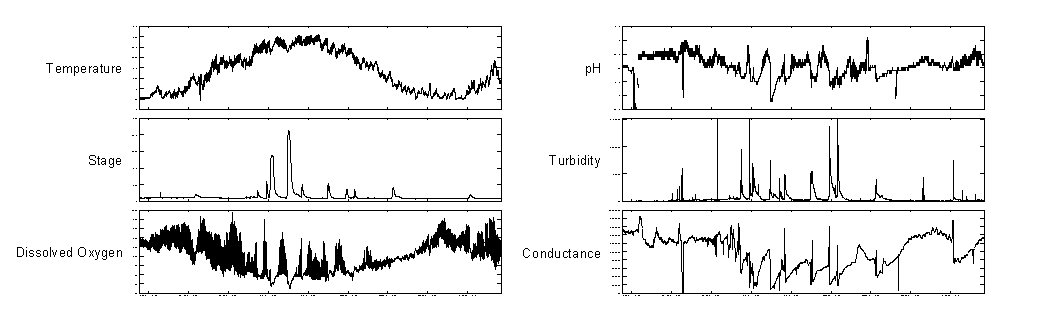
\includegraphics[width=\textwidth, height=6cm]{watermonitoring.eps}
\end{center}
\caption{16 months worth of data from six representative
signals in water quality monitoring,
which corresponds to approximately 11\,000 measurements per series.
These signals are highly nonlinear, demonstrating periodicity at
different scales,
intermittent pulses, and changes in dynamics. Not only do these
signals exhibit a wide range of dynamics,
but different signals of the same measurement type can also differ
drastically if they are taken in different regions. The figure also depicts typical problems with the data, including missing observations, outliers and discontinuities.
}
\label{fig:monitoring}
\end{figure*}


The collection of literature on fault- (also known as novelty-, anomaly-
and one-class-) detection is vast
\cite{Isermann2005, Ding2008,Markou2003,Chandola:2009,Khan2010,Dereszynski}.
Unfortunately, the problems solved by most of these techniques are of
very different character to our own, rendering such techniques
inapplicable. Further, after
much experimentation with those methods that are applicable (some of the results
appear in our experiments section) it became clear that off-the-shelf
techniques could not satisfy our requirements for reliable water
monitoring. This was predominately due to excessively restrictive assumptions
(e.g., that signals were linear, Markov or Gaussian), and/or a failure to
produce reasonable uncertainty
estimates. Green-tech areas, including environmental monitoring and
energy-demand prediction, are still far from full
automation; the provision of uncertainty estimates is necessary to
allow human operators to make appropriate decisions. For this reason,
we focus on developing probabilistic nonlinear models of the signal. In
addition to
providing posterior probabilities of observation faultiness, we are
able to perform effective prediction for the latent process even in
the presence of faults.

Our proposed method will rely on Gaussian processes (\acro{gp}s) due
to their flexibility and widely demonstrated effectiveness at modeling
nonlinear distributions. \acro{gp}s have been used previously for
fault detection in \citep{Eciolaza2001}, but in a very different
context, unsuitable for our problem. Previous work along similar lines
has approached this problem by creating observation models that
specify
the anticipated potential fault types \textit{a priori}
\citep{garnettosborne}, but this is usually an unreasonable assumption
in highly variable or poorly understood environments. 
In our proposed  ``fault bucket'' approach, we do not require the specification of precise fault models. In
this way, our model can simultaneously identify anomalies and robustly
make predictions in the presence of sensor faults. 
% Since we cannot
% make any strong assumptions about the nature of the faults, we model
% the faulty process as a distribution with extremely high variance.
The result is a fast and efficient method for data-stream prediction
that can manage a
wide range of faults without requiring significant
domain-specific knowledge.

\section{Fault Bucket}\label{bucket}
Gaussian processes provide a simple, flexible framework for performing
Bayesian inference about latent functions \citep{gpml}.  In
environmental monitoring, exact measurements of the latent function
are typically not available.
% however,
%  we may combine the Gaussian process distribution on the
% latent function with an observation model that takes into account
% potential noise in our measurements.  
Let $z(x)$ represent the value of an observation of the signal at $x$
and $y(x)$ represent the value of the unknown true latent signal at
that point.  When the observation mechanism is not expected to
experience faults, the usual noise model used is
\begin{equation}\label{iidnoise}
 p(z \given y, x, \sigma_n^2)
 \deq
 \cm{N}(z; y, \sigma_n^2),
\end{equation}
which represents additive i.i.d.\space Gaussian observation noise with
variance $\sigma_n^2$. Note that this model is inappropriate when
sensors can experience faults, which complicate the relationship
between $z$ and $y$.

Rather than specifying explicit parameters for every possible fault
type, we propose a single catch-all ``fault bucket'' that can identify
and treat appropriately measurements that are suspected of being
faulty.  The basic idea is to model faulty observations as being
generated from a Gaussian distribution with a very wide variance;
points that are more likely under this model than under the normal
predictive model of the Gaussian process can reasonably be assumed to
be corrupted in some way, assuming we have a good understanding of the
latent process. It is hoped that a very broad class of faults can be
captured in this way. To formalize this idea, we choose an observation noise distribution to
replace that in \eqref{iidnoise} that models the noise as independent
but not identically distributed with separate variances $\sigma_n^2$ and $\sigma_f^2$ for the
non-fault and fault cases.

\begin{figure*}
  \centering
  \small
  \psff{painting_big} \\
  \psff{fishkiller}
  \caption{Mean and $\pm3\sigma$ standard-deviation bounds for the
    predictions of the fault-bucket algorithm on (top), the painting
    dataset and (bottom), the ``fishkiller'' dataset.}
  \label{justfb}
\end{figure*}

\begin{figure*}
  \centering
  \small
  \psff{bias} \\
  \psff{dynamics}
  \caption{Mean and $\pm3\sigma$ standard-deviation bounds for the
    predictions of the fault-bucket algorithm on (top), a synthetic
    bias fault and (bottom), a synthetic change-in-dynamics fault.
    Detected faults are marked in black crosses, and the unobserved
    true values are marked in grey circles.}
  \label{synthetic}
\end{figure*}

% We make four key approximations:
% \begin{enumerate}
%  \item \label{app:fb} {\bf Fault bucket:} Faulty observations are assumed to be generated from a Gaussian noise distribution with a very wide variance.
% \item \label{app:single_gaussian} {\bf Single-Gaussian marginal:} A mixture of Gaussians, weighted by the posterior probabilities of faultiness of old data, is approximated as a single moment-matched Gaussian.
% \item \label{app:independence} {\bf Old/new noise independence:} We assume that noise contributions are independent, and that the contributions for new data are independent of old observations.
% \item \label{app:affine} {\bf Affine precision:} The precision matrix over both old and new halves is assumed to be affine in the precision matrix over the old half.
% \end{enumerate}


% \begin{align*}
%  p(z \given y, x, \neg\fault, \sigma_n^2)
%  &
%  \deq
%  \cm{N}(z; y, \sigma_n^2)
%  \\
%  p(z \given y, x, \fault, \sigma_f^2)
%  &
%  \deq
%  \cm{N}(z; y, \sigma_f^2),
% \end{align*}
% where $\fault \in \lbrace 0, 1 \rbrace$ is a binary indicator of
% whether the observation $z(x)$ was faulty and $\sigma_f > \sigma_n$ is
% the standard deviation around the mean of faulty measurements.  
% % The
% values of both $\sigma_n$ and $\sigma_f$ form hyperparameters of our
% model and are hence included in $\theta$.

Of course, {\it a priori}, we do not know whether any given
observation will be faulty.  Unfortunately, managing our uncertainty
about the ``faultiness'' of all available observations is a
challenging task. With $N$ observations available, there are $2^N$
possible assignments of faultiness. It quickly becomes computationally infeasible to marginalize over all these possible values. Instead, we approximate our marginal predictions, a sum of Gaussians weighted by the posterior probabilities of faultiness of old data, as a single moment-matched Gaussian. In order to effect this approximation, we adopt a sequential approach, applicable for ordered data
such as time series. For time series, the value to be predicted $y\st$ typically lies in the future; we can hence assume that the faultiness of old observations is less pertinent than that of newer observations. At any point in time, then, we approximately resolve our sum over faultiness 
by representing
each observation as having a known variance lying between between
$\sigma_n^2$ and $\sigma_f^2$.
 The more likely an observation's
faultiness, the closer its assigned variance will be to the (large)
fault variance and the less relevant it will become for inference
about the latent process. This approximate observation is then used
for future predictions; we need never consider the full sum over all
observations. Nonetheless, this approximate marginalization over
faultiness is preferable to heuristics that would designate all
observations as either faulty or not; our method acknowledges the
uncertainty that may exist in our belief about faultiness.

 The further mathematical details of our approximations are not
reproduced here for brevity.
%% So, we take
%% \begin{align*}
%%  &\p{y\st}{\data_{a}} \simeq \cm{N}\bigl(y\st; \amean{y\st}{\data_a}, \acov{y\st}{\data_a}\bigr),%\label{eq:pya}
%% \end{align*}
%% where we have
%% \begin{align}
%% \amean{y\st}{\data_{a}} \defequal {}& K_{\star,a} \tilde{V}_a^{-1} \vz_a,\label{eq:ameana}\\
%% \acov{y\st}{\data_{a}}
%% \defequal {}& K_{\star,\star} - K_{\star,a}(\tilde{V}_a^{-1}-\tilde{W}_a^{-1})K_{a,\star} 
%% \nonumber\\
%% & - \amean{y\st}{\data_{a,b}}^2 ,\label{eq:acova}
%% \end{align}
%% where
%% \begin{align}
%%  \tilde{V}_a^{-1}  & \defequal \sum_i \Prob{\vs^i_{a}}{\data_a} (V_a^i)^{-1},\nonumber\\
%%  \tilde{W}_a^{-1} & \defequal \sum_i \Prob{\vs^i_{a}}{\data_a} (V_a^i)^{-1}\vz_a \vz_a^\tr (V_a^i)^{-1}.\label{eq:Wa}
%% \end{align}
%% Note that for $\tilde{W}_a$, explicitly computing (unstable) matrix
%% inverses can be avoided by solving the appropriate linear equations
%% using Cholesky factors.  For $\tilde{V}_a$, we can rewrite
%% $(A^{-1}+B^{-1})^{-1} = A (A+B)^{-1} B$. If $i\in\{0,1\}$ (as it would
%% be if $a$ identified a single observation which could be either faulty
%% or not),
%% \begin{align} \label{eq:inverse_trick}
%% \tilde{V}_a & = V^0_a\bigl(
%% \Prob{\vs^1_{a}}{\data_a} V^0_a 
%% + 
%% \Prob{\vs^0_{a}}{\data_a} V^1_a
%% \bigr)^{-1}V^1_a.
%% \end{align}
%% If $i$ takes more than two values, we can simply iterate using the
%% same technique. Having used \eqref{eq:inverse_trick} to compute
%% $\tilde{V}_a$, we can then calculate
%% \begin{align*}
%%  \tilde{R}_a & \defequal \chol \tilde{V}_a \\%\label{eq:Ra}, \\
%%  \tilde{T}_a & \defequal \chol (\tilde{R}_a)^{-1} \vz_a %\label{eq:Ta},
%% \end{align*}
%% and use them, along with \eqref{eq:Wa}, to efficiently determine
%% \eqref{eq:ameana} and \eqref{eq:acova}.

%% Now, with these calculations performed, we can imagine receiving
%% further data $\data_b$. Our predictions are now
%% \begin{align*}
%% \p{y\st}{\data_{a,b}} & = \sum_{i} \sum_{j} \p{y\st}{\data_{a,b}, \vs^{i,j}_{a,b}} \Prob{\vs^{i,j}_{a,b}}{\data_{a,b}}.
%% \end{align*}
%% The full sums here can easily become too large to actually
%% evaluate. To simplify, we assume that our later observations are
%% independent of the noise in our earlier observations. To be precise, we approximate as
%% \begin{align} \label{eq:approx}
%% \Prob{\vs^{i,j}_{a,b}}{\data_{a,b}} & \simeq \Prob{\vs^i_{a}}{\data_a}\,\Prob{\vs^j_{b}}{\data_{a,b}},
%% \end{align}
%% giving
%% \begin{align}
%% p(y\st \given& \data_{a,b}) &\nonumber\\
%% \simeq {}& \sum_{j} \Prob{\vs^j_{b}}{\data_{a,b}}\sum_{i} \Prob{\vs^i_{a}}{\data_a} \p{y\st}{\data_{a,b}, \vs^{i,j}_{a,b}}\nonumber\\
%% = {}&\sum_{j} \Prob{\vs^j_{b}}{\data_{a,b}}\sum_{i} \Prob{\vs^i_{a}}{\data_a}\times {}\nonumber 
%% \\
%% & \cm{N}\bigl(y\st; \mean{y\st}{\data_{a,b}, \vs^{i,j}_{a,b}}, \cov{y\st}{\data_{a,b}, \vs^{i,j}_{a,b}}\bigr).\label{eq:sum_o_Gaussians}
%% \end{align}
%% Before trying to manage these sums, we will determine $p(\vs_b \given
%% \data_{a,b})$. As before, this distribution gives us the probability
%% of the observations $\data_b$ being faulty. For example, if we have
%% only a single observation $\data_b$, $
%% p\bigl(\fault(\data_b) \given \data_{a,b}\bigr) = \Prob{\sigma_b =
%%   \sigma_f}{\data_{a,b}} $. We define
%% \begin{align*}
%% \amean{\vz_b}{\data_a} \defequal {} &
%% K_{b,a} \tilde{V}_a^{-1} \vz_a %\label{eq;ameanba}
%% \\
%% \acov{\vz_b}{\data_{a},\vs_b}
%% \defequal {} & V_b - K_{b,a}(\tilde{V}_a^{-1}-\tilde{W}_a^{-1})K_{a,b}
%% \nonumber\\
%% & - \amean{\vz_b}{\data_{a,b}}^2, %\label{eq;acovba}
%% \end{align*}
%% where both $\tilde{V}_a$ (or its Cholesky factor) and
%% $\tilde{W}_a^{-1}$ were computed previously. By using
%% \eqref{eq:approx} and again approximating a sum of Gaussians as a
%% single Gaussian,
%% \begin{align*}
%% \Prob{\vs_b}{\data_{a,b}} & = \frac{\sum_i \p{\vz_b}{\data_a,\vs^i_{a,b}}p(\vz_a,\vs^i_{a,b})}{p(\vz_{a,b})}\nonumber\\
%% & \simeq \frac{\sum_i \p{\vz_b}{\data_a,\vs^i_{a,b}}\fPr(\vs_a^i\mid{\data_a})\fPr(\vs_{b})}{\ps{\vz_{b}}{\data_a}}\nonumber\\
%% & \simeq \frac{\cm{N}\bigl(\vz_b; \amean{\vz_b}{\data_a}, \acov{\vz_b}{\data_a, \Sigma_b}\bigr) \fPr(\vs_b)}{\p{\vz_{b}}{\data_a}},%\label{eq:psb}
%% \end{align*}
%% where we have
%% \begin{align}
%% p(\vz_{b} &\given \data_a)\nonumber\\
%% & = \sum_i \sum_j \p{\vz_b}{\data_a,\vs^i_{a,b}}\Prob{\vs^{i,j}_{a,b}}{\data_a}\nonumber\\
%% & \simeq \sum_i \sum_j \p{\vz_b}{\data_a,\vs^i_{a,b}}\Prob{\vs_a^i}{\data_a}\fPr(\vs_{b}^j)\nonumber\\
%% & \simeq \sum_j \cm{N}\bigl(\vz_b; \amean{\vz_b}{\data_a}, \acov{\vz_b}{\data_a, \vs_b^j}\bigr) \fPr(\vs_b^j).\label{eq:likelihood_b}
%% \end{align}
%% Note that the product of \eqref{eq:likelihood_b} and
%% \eqref{eq:likelihood_a} gives the likelihood of our hyperparameters.
%% Now, returning to \eqref{eq:sum_o_Gaussians}, we will once again
%% approximate a sum of Gaussians as a moment-matched single
%% Gaussian. Our goal here is to reuse our previously evaluated sums over
%% $i$ to resolve future sums over $i$. As we gain more data, the
%% faultiness of very old data becomes less important. We arrive at
%% \begin{align}
%% \p{y\st}{\data_{a,b}} & \simeq \N{y\st}{\amean{y\st}{\data_{a,b}}}{\acov{y\st}{\data_{a,b}}}\,,\label{eq:pyab}
%% \end{align}
%% where we have
%% \begin{align*}
%% \amean{y\st}{\data_{a,b}} \defequal {}&  K_{\star,a,b} \tilde{V}_{a,b}^{-1} \vz_{a,b}%\label{eq:ameanab}
%% \\
%% \acov{y\st}{\data_{a}}
%% \defequal {} & K_{\star,\star} - K_{\star,a}(\tilde{V}_{a,b}^{-1}-\tilde{W}_{a,b}^{-1})K_{a,\star} {} \nonumber
%% \\
%% & - \amean{y\st}{\data_{a,b}}^2 \,.%\label{eq:acovab}
%% \end{align*}
%% where
%% \begin{align*}
%% \tilde{V}^{-1}_{a,b} \defequal {} &
%% \sum_{j} \Prob{\vs^j_{b}}{\data_{a,b}}\sum_i \Prob{\vs^i_{a}}{\data_{a}} (V_{a,b}^{i,j})^{-1} \\
%% \tilde{W}^{-1}_{a,b} \defequal {} &
%% \sum_{j} \Prob{\vs^j_{b}}{\data_{a,b}}\sum_i \Prob{\vs^i_{a}}{\data_{a}} (V_{a,b}^{i,j})^{-1}  
%% %\times {} 
%% \\
%% & \times \vz_{a,b}^{\phantom{\tr}} \vz_{a,b}^\tr (V_{a,b}^{i,j})^{-1}.
%% \end{align*}
%% Now, using the inversion by partitioning formula \citep[Section 2.7]
%% {NumericalRecipes},
%% \begin{align*}
%% \hspace{-0.2cm}&({V}^{i,j}_{a,b})^{-1} = \\
%% &\begin{bmatrix}
%%  S^{i,j}_a &\hspace{-0.1cm} -S^{i,j}_a K_{a,b} (V^j_b)^{-1} \\
%%  - (V^j_b)^{-1} K_{b,a} S^{i,j}_a &\hspace{-0.1cm} (V^j_b)^{-1}\!+\!(V^j_b)^{-1} K_{b,a} S^{i,j}_a K_{a,b} (V^j_b)^{-1} 
%% \end{bmatrix},
%% \end{align*}
%% where
%% $
%% S^{i,j}_a \defequal (V^i_a -K_{a,b} (V^j_b)^{-1}K_{b,a})^{-1}\,.
%% $

%% Note that $({V}^{i,j}_{a,b})^{-1}$ is affine in $S^{i,j}_a$, so that when
%% \begin{equation}\label{eq:V_a_big}
%%  V_a \gg K_{a,b} V_b^{-1} K_{b,a}\,,
%% \end{equation}
%% $({V}^{i,j}_{a,b})^{-1}$ is effectively affine in $(V^i_a)^{-1}$. This
%% is true if given $\data_b$, it is impossible to accurately predict
%% $\data_a$. This might be the case if $\data_a$ represents a lot of
%% information relative to $\data_b$ (if, for example, $\data_a$ is our
%% entire history of observations where $\data_b$ is simply the most
%% recent observation), or if $\data_b$ and $\data_a$ are simply not
%% particularly well correlated. On this basis, \eqref{eq:V_a_big} seems
%% reasonable for our application. Defining the affine map $f\colon (V^i_a)^{-1}
%% \mapsto ({V}^{i,j}_{a,b})^{-1}$, then, noticing $\sum_i \Prob{\vs^i_{a}}{\data_{a}} = 1$,
%% $$
%% \sum_i \Prob{\vs^i_{a}}{\data_{a}} f\bigl((V^i_a)^{-1} \bigr) \simeq f\Bigl(\sum_i \Prob{\vs^i_{a}}{\data_{a}}(V^i_a)^{-1} \Bigr).
%% $$
%% Therefore, for
%% \begin{align*}
%% \hat{V}^{j}_{a,b} & \defequal
%% \begin{bmatrix}
%%  \tilde{V}_a & K_{a,b}
%% \\
%%  K_{b,a} & V^j_b
%% \end{bmatrix},
%% \\
%% %\ 
%% \tilde{V}^{-1}_{a,b} &\simeq \sum_j \Prob{\vs^j_{b}}{\data_{a,b}} (\hat{V}^{j}_{a,b})^{-1},
%% \nonumber\\
%% \tilde{V}_{a,b} & \simeq
%% \begin{bmatrix}
%%  \tilde{V}_a & K_{a,b}\\
%%  K_{b,a} & \tilde{V}_{b|a} + K_{b,a} \tilde{V}_a^{-1} K_{a,b}
%% \end{bmatrix},
%% \end{align*}
%% where
%% \begin{equation*}
%%  \tilde{V}^{-1}_{b|a} \defequal \sum_j \Prob{\vs^j_{b}}{\data_{a,b}} (V^j_b -K_{b,a} \tilde{V}_a^{-1}K_{a,b})^{-1}
%% \end{equation*}
%% can be computed using the same trick as in \eqref{eq:inverse_trick} if
%% $b$ identifies a single observation and $j\in\{0,1\}$. Note that the
%% lower right hand element of $\tilde{V}_{a,b}$ defines the noise
%% variance to be associated with observations $\data_b$. As before, we
%% determine our predictions \eqref{eq:pyab} by solving linear equations
%% using the quantities
%% \begin{align}
%%  \tilde{R}_{a,b} & \defequal \chol \tilde{V}_{a,b} \label{eq:Rab}, \\
%%  \tilde{T}_{a,b} & \defequal \chol (\tilde{R}_{a,b})^{-1} \vz_a \label{eq:Tab};
%% \end{align}
%% both of which can be efficiently determined \citep[Appendix
%%   B]{osbornebayesian} using the evaluated $\tilde{R}_a$ and
%% $\tilde{T}_a$.

%% We now turn to $\tilde{W}_{a,b}^{-1}$. Unfortunately, even if
%% \eqref{eq:V_a_big} were true, $\tilde{W}_{a,b}^{-1}$ is quadratic in
%% $(V^i_a)^{-1}$. We will nonetheless assume that $\tilde{W}_{a,b}^{-1}$
%% is affine in $(V^i_a)^{-1}$. The quality of our approximation for
%% $\tilde{W}_{a,b}^{-1}$ is much less critical than for
%% $\tilde{V}^{-1}_{a,b}$, because the former only influences the
%% variance of our predictions for the current predictant; any flaws in
%% that approximation will not be propagated forward. Further, of course,
%% if one probability dominates, 
%% \begin{equation*}
%% \Prob{\vs^i_{a}}{\data_{a}}\gg
%% \Prob{\vs^{i'}_{a}}{\data_{a}} \quad \forall i' \neq i,
%% \end{equation*} 
%% then the approximation is valid. With this,
%% \begin{align}
%% \tilde{W}^{-1}_{a,b} \defequal
%% & \sum_{j} \Prob{\vs^j_{b}}{\data_{a,b}} (\hat{V}_{a,b}^{j})^{-1}\vz_{a,b}^{\phantom{\tr}} \vz_{a,b}^\tr (\hat{V}_{a,b}^{i,j})^{-1}\,.\label{eq:Wab}
%% \end{align}
%% and we can solve for
%% $K_{\star,(a,b)}\tilde{W}^{-1}_{a,b}K_{(a,b),\star}$ by efficiently
%% updating using the previously computed quantity $\tilde{T}_{a}$.

%% \begin{algorithm}[tb]
%%    \caption{Fault Bucket}
%% \label{alg:fault_bucket}
%% \begin{algorithmic}
%%    \STATE {\bfseries input:} data $(\vx,\vz)$, lookahead $\delta$
%% \STATE $x_a \leftarrow x_1,\, z_a \leftarrow z_1,
%% \,x\st \leftarrow x_{1+\delta}$
%% \\
%% \STATE {\bfseries return:} $p(\vz_a) \leftarrow$\eqref{eq:likelihood_a}
%% \FOR {$i = 0,1$}
%% \STATE {\bfseries return:} $\Prob{\vs^i_a}{\data_{a}} \leftarrow$ \eqref{eq:psa}\\
%% \ENDFOR
%%  \STATE $\tilde{R}_a \leftarrow$ \eqref{eq:Ra}, $\tilde{T}_a\leftarrow$ \eqref{eq:Ta}, \, $\tilde{W}^{-1}_a \leftarrow$ \eqref{eq:Wa}\\
%%  \STATE $\amean{y\st}{\data_a} \leftarrow$ \eqref{eq:ameana}, $\acov{y\st}{\data_a} \leftarrow$ \eqref{eq:acova}\\
%% \STATE {\bfseries return:} $\p{y\st}{\data_{a}} \leftarrow$ \eqref{eq:pya}\\
%% \FOR {$t = 2,\ldots$}
%% \STATE $x_b \leftarrow x_t, z_b \leftarrow z_t, x\st \leftarrow x_{t+\delta}$\\
%% \STATE $\amean{\vz_b}{\data_a} \leftarrow$ \eqref{eq;ameanba}, $\acov{\vz_b}{\data_a} \leftarrow$ \eqref{eq;acovba}\\
%% \STATE $\p{\vz_b}{\data_a} \leftarrow$ \eqref{eq:likelihood_b}\\
%% \FOR {$j = 0,1$}
%% \STATE {\bfseries return:} $\Prob{\vs^j_b}{\data_{a,b}} \leftarrow$ \eqref{eq:psb}\\
%% \ENDFOR
%% \STATE $\tilde{R}_{a,b} \leftarrow$ \eqref{eq:Rab}, $\tilde{T}_{a,b}\leftarrow$ \eqref{eq:Tab}, \, $\tilde{W}^{-1}_{a,b} \leftarrow$ \eqref{eq:Wab}\\
%%  \STATE $\amean{y\st}{\data_{a,b}} \leftarrow$ \eqref{eq:ameanab}, $\acov{y\st}{\data_{a,b}} \leftarrow$ \eqref{eq:acovab}\\
%% \STATE {\bfseries return:} $\p{y\st}{\data_{a,b}}\leftarrow$ \eqref{eq:pyab}\\
%% \STATE {\bfseries return:} $p(\vz_a) \leftarrow p(\vz_a)\p{\vz_b}{\data_a}$
%% \STATE $x_a \leftarrow \{x_a,x_b\},\, z_a \leftarrow \{z_a,z_b\}$\\
%% \STATE $\tilde{R}_a \leftarrow \tilde{R}_{a,b},\, \tilde{T}_a\leftarrow \tilde{T}_{a,b}$\\
%% \ENDFOR 
%% \end{algorithmic}
%% \end{algorithm}

%% %% An outline of our approach is depicted in Algorithm \ref{alg:fault_bucket}.

%% \subsection{Discussion}

%% We will discuss briefly the management of hyperparamters, denoted
%% $\theta$. Unfortunately, analytically marginalizing $\theta$ is
%% impossible. Most of the hyperparameters of our model can be set by
%% optimizing their likelihood on a large training set, giving a
%% likelihood close to a delta function. This is not true of the
%% hyperparameters $\sigma_n$ and $\sigma_f$, due to exactly the same
%% problematic sums discussed earlier. Instead, we marginalize these
%% hyperparameters online using Bayesian Monte Carlo \citep[Chapter
%%   7]{osbornebayesian}, taking a fixed set of samples in their values
%% and using the hyperparameter likelihoods to construct weights over
%% them. Essentially, we proceed as described above independently in
%% parallel for each sample, and combine the predictions from each in a
%% final weighted mixture for prediction. Note that we can use a similar
%% procedure \citep{garnettosborne} to determine the full posterior
%% distributions of $\sigma_n$ and $\sigma_f$, if desired.  It would be
%% desirable to use non-fixed samples, but, unfortunately, this would
%% require reconstructing our full covariance matrix from scratch each
%% time a sample is moved.

%% Our proposed algorithm steps through our data one at a time, so that
%% $\data_b$ always contains only a single observation. However, it would
%% be possible in general to step in larger chunks, evaluating larger
%% sums. Although more computationally demanding, this might be expected
%% to improve results. It would also allow us to consider non-diagonal
%% noise contributions.

%% We have so far not specified our prior for faultiness (as expressed by
%% $p(\sigma_a)$ and $p(\sigma_b)$). Within this paper, we consider
%% exclusively a time-independent probability of faultiness. However,
%% within the framework afforded by our approximation \eqref{eq:approx},
%% we are free to consider noise variances that are expected to change
%% over time.

%% In some contexts it might be useful to perform inference about the
%% fault contribution, rather than the signal of interest.  This task is
%% trivial; we merely switch the roles of the fault and non-fault
%% contributions. Note that, using our full posteriors for faultiness, we
%% can also trivially use Bayesian decision theory to make hard decisions
%% as required.
%% % To make a prediction about a potential faulty signal
%% % at $x$, we follow exactly the same procedure as above, substituting
%% % $\sigma_n^2$ for $\sigma_f^2$.

%% \begin{figure*}
%%   \centering
%%   \small
%%   \psff{bias}
%%   \psff{kf_bias}
%%   \vspace*{2\baselineskip}
%%   \psff{dynamics}
%%   \psff{kf_dynamics}
%%   \caption{Mean and $\pm3\sigma$ standard-deviation bounds for the
%%     predictions of (first and third) the fault-bucket algorithm and
%%     (second and fourth) the Kalman filter algorithm on (top two) the
%%     synthetic bias dataset and (bottom two), the synthetic anomaly
%%     dataset.  Detected faults are marked in black crosses, and the
%%     unobserved true values are marked in grey circles.}
%%   \label{compare}
%% \end{figure*}

\begin{table*}
  \begin{center}
  \caption{Quantitative comparison of different algorithms on datasets with two simulated faults.  For each dataset, we show the mean squared error
    (\textsc{mse}), the log likelihood of the true data ($\log p(\bm{y}
    \given \bm{x})$), and the true-positive and false-positive rates
    of detection for faulty points (\textsc{tpr} and \textsc{fpr}),
    respectively, with all methods permitted a `burn-in' period of 50 points. The best value for each set of results is highlighted in
    bold.}
    \vspace{2mm}
  \label{tbl:results}
  \begin{tabular}{ccccccccc}
    \toprule
& \multicolumn{4}{c}{Bias dataset} & \multicolumn{4}{c}{``Flash-flood'' dataset}\\
    \cmidrule(l){2-5} \cmidrule(l){6-9}
    Method & \scshape{mse} & $\log p(\bm{y}\given\bm{x})$ & \scshape{tpr} & \scshape{fpr} 
& \scshape{mse} & $\log p(\bm{y}\given\bm{x})$ & \scshape{tpr} & \scshape{fpr} \\
\midrule
    \scshape{fb} & \textbf{0.024} & 334 & \textbf{0.997} & 0.031 & 0.069 & $-5.77\times 10^3$ & \textbf{0.829} & {0.016} \\
    \scshape{xgp} & 0.037 & \textbf{439} & 0.982 & \textbf{0.022} & \textbf{0.042} & $\mathbf{-1.52 \times 10^3}$ & 0.805 & \textbf{0.012} \\
    \scshape{tgp} & 0.033 & 278 & \textbf{0.997} & 0.031 & 0.075 & $-8.29\times 10^3$ & \textbf{0.829} & 0.083 \\
%    \scshape{argp} & 2.340 & $-1.93 \times 10^9$ & 0.6 & 0.4 & 1.097 & $-7.52\times 10^8$ & 0.178 & 0.822 \\
    \scshape{mlh} & 0.940 & $-5.43\times 10^7$ & 0.065 & 0.031 & 2.369 & $-2.27\times 10^7$ & 0.045 & 0.262 \\
%    \scshape{kf} & 0.894 & $-7.11 \times 10^5$ & 0.053 & 0.073 & 0.360 & $-3.54 \times 10^4$ & 0.835 & 0.046 \\
   \scshape{ekf} & 0.060 & $-1.26 \times 10^4$ & 0.551 & 0.258 & 0.613 & $-1.81\times 10^4$ & 0.169 & 0.768 \\
    \bottomrule
  \end{tabular}
  \end{center}
\end{table*}

%% % Finally, some applications might required a hard decision about
%% % whether a particular observation was faulty.  This would be necessary,
%% % for example, if a system had correctional or responsive actions that
%% % it could take when such an event occurred.  Fortunately, we can
%% % address this problem using simple Bayesian decision theory.

\section{Results}
%\subsection{Results}
Figure \ref{justfb} shows the performance of the fault-bucket
algorithm on the two real datasets.  The first dataset contains a
fault type called ``painting,'' which is an error that occurs when ice
builds on a sensor obscuring some of the readings. It is characterised
by frequent sensor spikes interlaced with the original, and still
accurate, signal.  Our second dataset, which we dub ``fishkiller'',
comes from a sensor near a dam on a river in British Columbia,
Canada. It contains an otherwise normal water level-reading that is
occasionally interrupted by a short period of rapid oscillation. This
occurs when dam operators open and close the floodgates too quickly,
leading to rapid water level drops followed by salmon becoming
stranded and suffocating. Detecting these events is critical to proper
regulation of dams. It is however a difficult problem as often these
events occur during other transitions.


Figure \ref{justfb} shows that, in both cases, the fault-bucket
algorithm is able to detect these markedly different types of
pattern. It is also capable of making accurate predictions.

Figure \ref{synthetic} shows the results of the fault-bucket algorithm
on two additional sustained faults that were created artificially from
real data, allowing the predictions made by the algorithm throughout
the fault period to be compared with the now-known (but unobserved by
the algorithm) ground truth.  The fault-bucket algorithm again
performs well, despite the very different nature of the faults.

We also tested against a number of different methods in order to establish the efficacy of the fault bucket algorithm. All \acro{gp}-based approaches used the same hyperparameters employed by our algorithm. The training set used to learn those hyperparameters was also supplied to other methods for their respective model learning phases. Several methods identify a new observation $y$ as a fault if
\begin{equation}
 \bigl\lvert y-\mean{y}{\vy} \bigr\rvert > 3\sigma_T\,,
 \label{eq:thresh}
\end{equation}
where $\mean{y}{\vy}$ is the method's \emph{a priori} prediction for $y$, and $\sigma_T$ is the noise standard deviation on the faultless training set. Of course, methods using \eqref{eq:thresh} or similar can not provide the posterior probability of a point's faultiness, as our algorithm can. Methods tested include:

%\begin{description}
%\item[ XGP] 
{\bf XGP:}
A  \acro{gp} in which we exhaustively search over the faultiness of the last 10 points, and approximate the noise variance of all previous points in the window as having the value $\sigma_f^2 \p{\fault}{\vy} + \sigma_n^2 \p{\neg\fault}{\vy}$, fixed at the time the point was observed (when data $\data$ was available). Clearly, this method is very much more computationally expensive than the fault bucket algorithm (roughly $2^9$ times more), but offers a useful way to quantify the influence of our approximations.

% \item[ TGP] 
{\bf TGP:}
A \acro{gp} in which a point was flagged as a fault using \eqref{eq:thresh}; if faulty, a point was treated as having noise variance $\sigma_f^2$.

%  \item[ ARGP] An auto-regressive Gaussian process (over the last 10 points), with a point identified as faulty using \eqref{eq:thresh}. If faulty, the value for the observation $y$ is taken as $\mean{y}{\vy}$ for future predictions.

%\item[MLH] 
{\bf MLH:} 
The most likely heteroscedastic  \acro{gp} \citep{kersting2007most}. Note that for this method we perform retrospective prediction (so that all data is available to make predictions about even the first predictant), as the method is intended to be used. Clearly this allows the method a predictive advantage relative to sequential methods, and the multiple passes over the data effected by \acro{mlh} cannot be readily applied to the sequential problem without requiring a great deal of expensive computation. 
%  \item[KF] A Kalman filter to perform one-step-lookahead predictions in an online fashion. Any datum identified as a fault by the threshold \eqref{eq:thresh} is simply ignored and discarded.

{\bf EKF:}
%\item[EKF] 
An autoregressive neural net trained with the extended Kalman filter to capture nonstationarity \cite{ndfEKF1,ndfEKF2}. Again, \eqref{eq:thresh} was used to identify and discard faulty data.
%\end{description}

Table \ref{tbl:results} displays quantitative measures of performance
for the various algorithms on datasets with two simulated faults. We used simulated faults provided by Aquatic Informatics in order to have access to ground-truth. The two faults are common in water monitoring. The results in the table indicate that,
in addition to superior predictive performance, our
detection rates for the faulty points are generally excellent. The results reveal that our algorithm is competitive with exhaustive search. Our na\"{i}ve approach to faults may, of course, suffer relative to better-informed models, but its probabilistic estimates provide a human operator with an indication as to whether more sophisticated analysis is necessary.

\section{Conclusion}
We have briefly presented an overview of some of the data challenges arising in water monitoring and sustainability. We demonstrated a novel algorithm, the ``fault bucket,'' for managing
time-series data corrupted by faults unknown ahead of time. The algorithm can also be used to detect other types of pattern, \emph{e.g.} ``fishkiller'' events, and produces probabilistic predictions. This not only results in an increase in automation, but also in sensible uncertainty summaries to assist human operators. On the machine learning front, our chief
contribution is a sequential method for marginalizing the
faultiness of observations in a \acro{gp} framework, allowing for
fast, effective prediction in the presence of unknown faults and the
simultaneous detection of faulty observations.

\section*{Acknowledgement}
The work reported in this paper was partly funded by the Systems
Engineering for Autonomous Systems (SEAS) Defence Technology Centre
established by the UK Ministry of Defence. We would like to thank the management and employees of Aquatic Informatics, and in particular Touraj Farhmand, for their support in this project.
All datasets have been provided by Aquatic Informatics. The data may
be obtained by contacting Touraj Farahmand at
\texttt{tourajf@aquaticinformatics.com}. 


\bibliography{fault_bucket_icml_2011}
\bibliographystyle{icml2011}

\end{document}


